\chapter{Guía de usuario}
\label{chap:guía de usuario}

\section{Interfaz gráfica}

Una interfaz gráfica de usuario (GUI) presenta un mecanismo amigable al usuario para interactuar con una aplicación. Una GUI proporciona a una aplicación una ``apariencia visual'' única. Al proporcionar distintas aplicaciones en las que los componentes de la interfaz de usuario sean consistentes e intuitivos, los usuarios pueden familiarizarse en cierto modo con una aplicación, de manera que pueden aprender a utilizarla en menor tiempo y con mayor productividad.\\

Las GUIs se crean a partir de componentes de la GUI. A éstos se les conoce también como controladores o widgets (accesorios de ventana) en otros lenguajes. Un componente de la GUI es un objeto con el cual interactúa el usuario mediante el ratón, el teclado u otra forma de entrada, como el reconocimiento de voz.\\

\section{Componentes GUI en java}

En java existen realmente dos conjuntos de componentes de GUI. Antes de introducir a Swing en Java SE 1.2, las GUIs de Java se creaban a partir de componentes del \textbf{Abstract Window Toolkit (AWT}) en el paquete \textbf{java.awt}. Cuando una aplicación de Java con una GUI del AWT se ejecuta en distintas plataformas, los componentes de la GUI de la aplicación se muestran de manera distinta en cada plataforma. Consideremos una aplicación que muestra un objeto de tipo \emph{Button} (paquete \emph{java.awt}). En una computadora que ejecuta el sistema operativo Microsoft Windows, el objeto \emph{Button} tendrá la misma apariencia que los botones en las demás aplicaciones Windows. De manera similar, en una computadora que ejecuta el sistema operativo Apple Mac OS X, el objeto \emph{Button} tendrá la misma apariencia visual que los botones en las demás aplicaciones Macintosh. Algunas veces, la forma en la que un usuario puede interactuar con un componente específico del AWT difiere entre una plataforma y otra.\\

En conjunto, a la apariencia y la forma en la que interactúa el usuario con la aplicación se les denomina la \textbf{apariencia visual}. Los componentes de GUI de Swing nos permiten especificar una apariencia visual uniforme para una aplicación a través de todas las plataformas, o para usar la apariencia visual personalizada de cada plataforma. Incluso, hasta una aplicación puede modificar la apariencia visual durante la ejecución, para permitir a los usuarios elegir su propia apariencia visual preferida.\\

%%PROVISIONAL HAY QUE REDACTARLO MEJOR

\section{Introducción}

En este documento se describirá los objetivos e información clara y concisa de cómo utilizar la Suite de Teoría Algorítmica de grafos: Graphvisualx.\\

La Suite de Teoría Algorítmica de grafos: Graphvisualx ha sido creado por Moisés Gautier Gómez para el proyecto de fin de carrera de la titulación de ingeniería informática técnica de sistemas de la universidad de Cádiz. El objetivo es facilitar en la compresión de los estudiantes de la materia de grafos en la resolución de ejemplos de los mismos empleando los algoritmos más conocidos y que usualmente se emplean en el entorno académico.\\

Es de mucha importancia consultar esta guía antes y/o durante la utilización de la Suite, ya que lo guiará paso a paso en el manejo de las funciones de ella.\\

Con el fin de facilitar la comprensión de la guía, se incluye gráficos explicativos.\\

\section{Objetivo de esta guía}

El objetivo primordial de esta guía es ayudar y guiar al usuario a utilizar la Suite de Teoría Algorítmica de grafos: Graphvisualx obteniendo la información adecuada de los algoritmos para despejar todas las dudas existentesy comprende:

\begin{itemize}
\item Guía para acceder a la Suite.
\item Conocer como utilizar la Suite, mediante una descripción detallada e ilustrada de opciones.
\item Conocer el alcance de todos los algoritmos por medio de una explicación detallada de ellos e ilustrada en el manual de algoritmos que se adjuntará en la guía y que también será accesible desde la Suite.
\end{itemize}

\section{Dirigido a}

Esta guía esta dirigida al usuario final de la Suite que utilicen dicho recurso como complemento al material docente de asignaturas de la titulación así como laboratorio de pruebas de algoritmos sobre grafos de ejemplo.

\section{Convenciones y estándares a utilizar}

Entre las convenciones y estándares a utilizar tenemos las siguientes:

\subsection{Convenciones del uso del ratón}

\begin{table}[H]
\begin{tabular}{|p{2cm}|p{3cm}|p{5cm}|p{5cm}|}
\hline
\centering{Término} & \centering{Situación} & \centering{Elemento aplicación} & \qquad \quad Significado \\
\hline
\centering{
\includegraphics[scale=.6]{./imagenes_documentacion/mouse.png}} & - & Sobre cualquier botón & Apertura del menú o acción designado para tal botón. \\
\hline
\multicolumn{4}{|c|}{Modo edición grafo} \\
\hline
\centering{
\includegraphics[scale=.6]{./imagenes_documentacion/mouse_left.png}} & Sobre lienzo de trabajo & Modo crear nodos sobre el lienzo (Botón crear nodo previamente pulsado). & Crea un nodo en el espacio designado para ello. \\
\hline
\centering{
\includegraphics[scale=.6]{./imagenes_documentacion/mouse_right.png}} & Sobre nodo creado en el lienzo de trabajo & Modo crear nodo sobre el lienzo (Botón crear nodo previamente pulsado). & Elimina el nodo creado anteriormente en el nodo. Se reorganiza la numeración del etiquetado de nodos si fuera necesario. \\
\hline
\centering{
\includegraphics[scale=.6]{./imagenes_documentacion/mouse_left.png}} & Sobre un nodo creado y arrastrar el cursor a otro nodo creado. Soltar inmediatamente. & Modo crear arista sobre el lienzo (Botón crear arista previamente pulsado). & Crea una arista de adyacencia (si es dirigido el grafo con la flecha de finalización apuntando hacia el nodo destino) sobre el nodo origen hacia el nodo destino. \\
\hline
\centering{
\includegraphics[scale=.6]{./imagenes_documentacion/mouse_right.png}} & Sobre una arista creada previamente (sobre la etiqueta de ponderación de la misma). & Modo crear arista sobre el lienzo (Botón crear arista previamente pulsado). & Da la opción de modificar el coste/ponderación de la arista o de eliminarla. \\
\hline
\centering{
\includegraphics[scale=.6]{./imagenes_documentacion/mouse_left.png}} & - & Modo eliminar contenido lienzo. & Elimina todos los elementos contenidos en el lienzo de trabajo. \\
\hline
\centering{
\includegraphics[scale=.6]{./imagenes_documentacion/mouse_both.png}} & Sobre un nodo creado en el lienzo de trabajo & Modo mover nodos (Botón mover nodos previamente pulsado) & Permite cambiar de posición el nodo dentro de lienzo según las preferencias del usuario. \\
\hline
\end{tabular}
\end{table}

\begin{table}[H]
\begin{tabular}{|p{2cm}|p{3cm}|p{5cm}|p{5cm}|}
\hline
\centering{
\includegraphics[scale=.6]{./imagenes_documentacion/mouse_left.png}} & - & Modo aceptar grafo & Concluye la edición del lienzo de trabajo para la creación de un grafo. \\
\hline
\end{tabular}
\end{table}
\vspace*{-.5in}{
\subsection{Convenciones del uso del teclado}}

\begin{table}[H]
\begin{center}
\begin{tabular}{|p{6cm}|p{8cm}|}
\hline
\centering{Tecla} & \qquad \quad Significado \\
\hline

\includegraphics[width=5.5cm]{./imagenes_documentacion/key_ctrl_g.png} & \vspace*{-.8in}{Guardar el grafo inicial. Abre un menú emergente en donde te permite guardar un fichero en formato texto plano en el sistema con el nombre que se desee. No hay que escribir explícitamente la extensión al definir el nombre del fichero, es decir, con escribir ``ejemplo'' el sistema asigna la extensión al nombre inmediatamente.} \\
\hline

\includegraphics[width=5.5cm]{./imagenes_documentacion/key_ctrl_x.png} & \vspace*{-.8in}{Salir de la Suite. Cierra la Suite y para volver a acceder a ella se tendrá que hacer doble clic sobre el lanzador.} \\
\hline
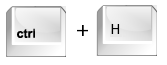
\includegraphics[width=5.5cm]{./imagenes_documentacion/key_ctrl_h.png} & \vspace*{-.8in}{Guía del usuario. Se abre una nueva ventana en donde vendrá definida la guía del usuario para cualquier duda sobre el uso de Graphvisualx.} \\
\hline

\includegraphics[width=5.5cm]{./imagenes_documentacion/key_ctrl_m.png} & \vspace*{-.8in}{Manual de los algoritmos y conceptos relacionados con la teoría algorítmica de grafos. Se abre una nueva ventana en donde vendrá definido un documento en formato pdf con los contenidos teóricos necesarios en caso de duda.} \\
\hline
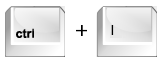
\includegraphics[width=5.5cm]{./imagenes_documentacion/key_ctrl_i.png} & \vspace*{-.8in}{Sobre Graphvisualx. Se abre una nueva ventana donde viene información sobre el autor de Graphvisualx y demás.} \\
\hline
\end{tabular}
\end{center}
\end{table}

\section{Ingreso al sistema}

Una vez descargada la aplicación y colocada en el directorio deseado hacemos doble clic sobre ella para ejecutar la Suite. Sino se produciese ningún evento probar con la siguiente opción:
\begin{figure}[H]
\hspace*{-.75in}{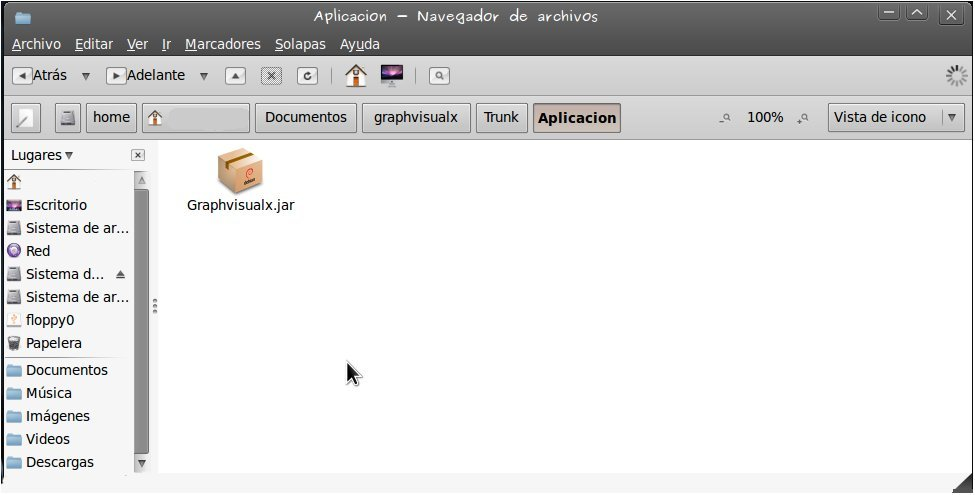
\includegraphics[width=20cm]{./imagenes_documentacion/captura_1.jpeg}}
\caption{Directorio de trabajo donde se encuentra el fichero .jar ejecutable de la Suite.}
\end{figure}

\begin{figure}[H]
\caption{PONER IMAGEN DE BOTON DERECHO AL PULSAR EL .JAR}
\end{figure}


\subsection{Como acceder a la suite}
\label{cap:Acceder}

Si no se dispusiese de máquina virtual java en el sistema se deberá instalar a través de línea de comandos en el terminal de GNU/Linux.
Para ello primeramente hay que escribir \url{http://www.java.com/es/download/help/linux_install.xml} en nuestro navegador favorito para ir a la página web de java, en donde se nos explica el método de instalación a seguir. Sea pues:

\begin{figure}[H]
\hspace*{-.8in}{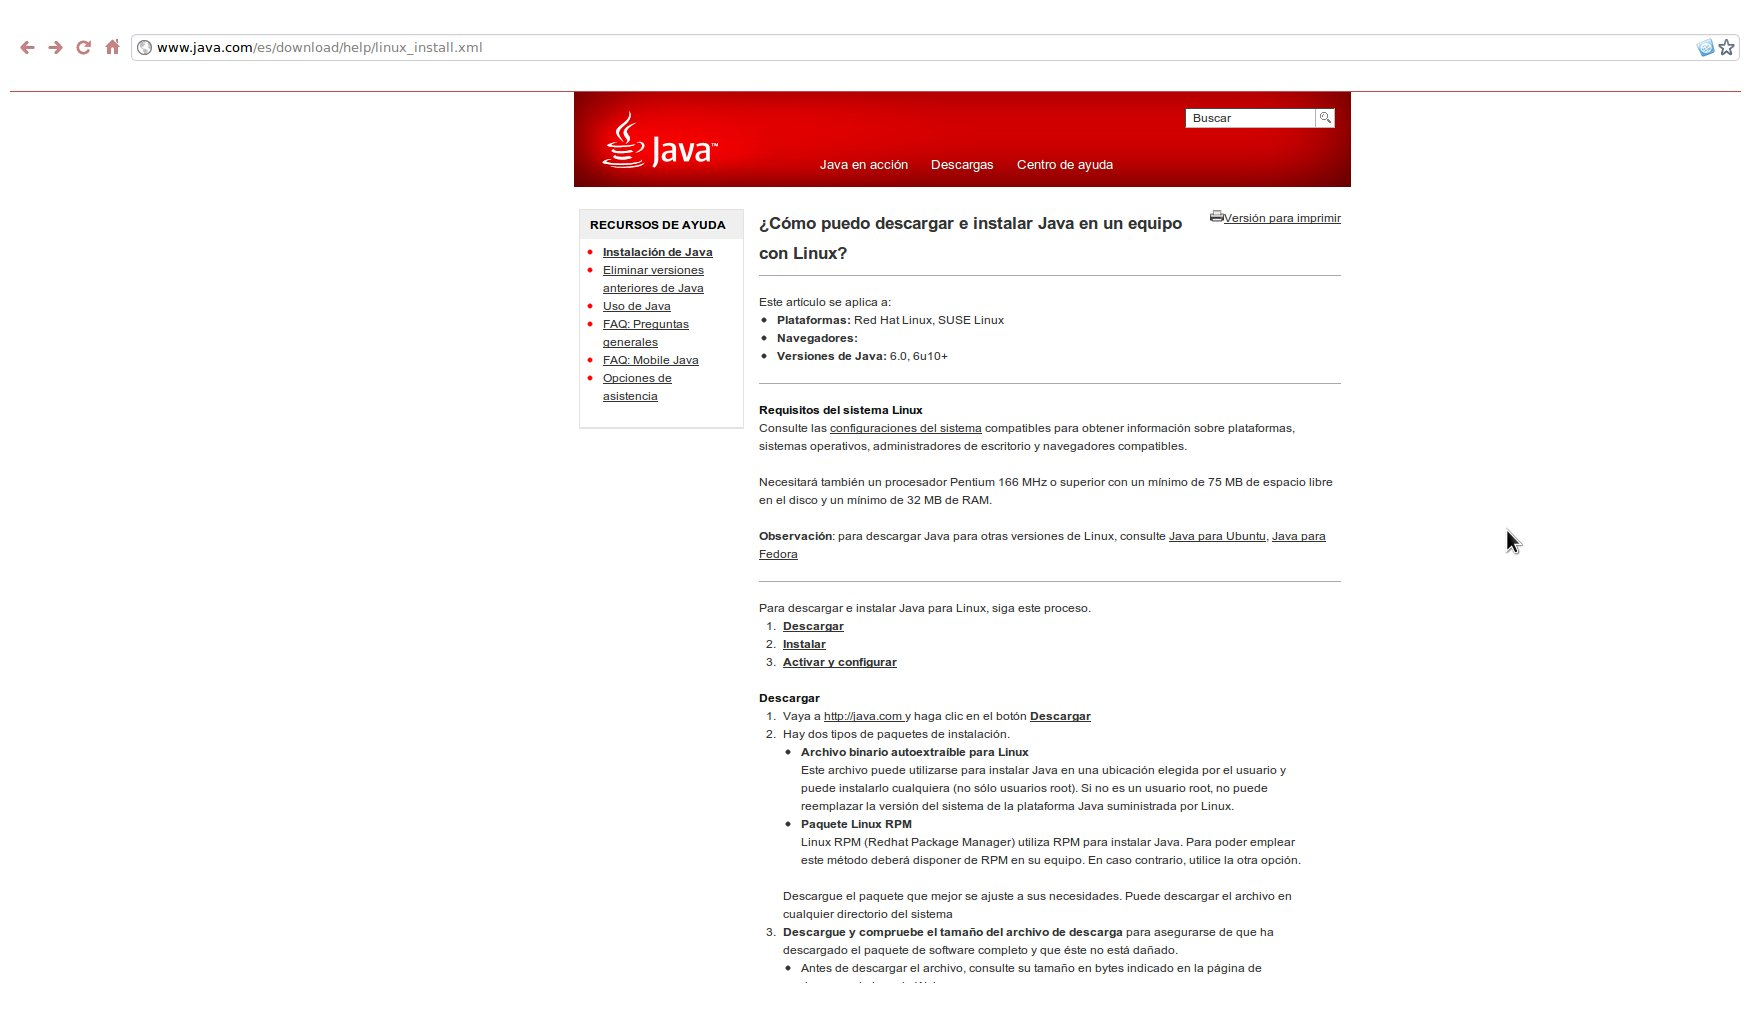
\includegraphics[width=20cm]{./imagenes_documentacion/captura_2.jpeg}}
\caption{Página web de Java donde se explican los pasos para la instalación del software Java en nuestro sistema GNU/Linux}
\end{figure}

\begin{figure}[H]
\hspace*{-.8in}{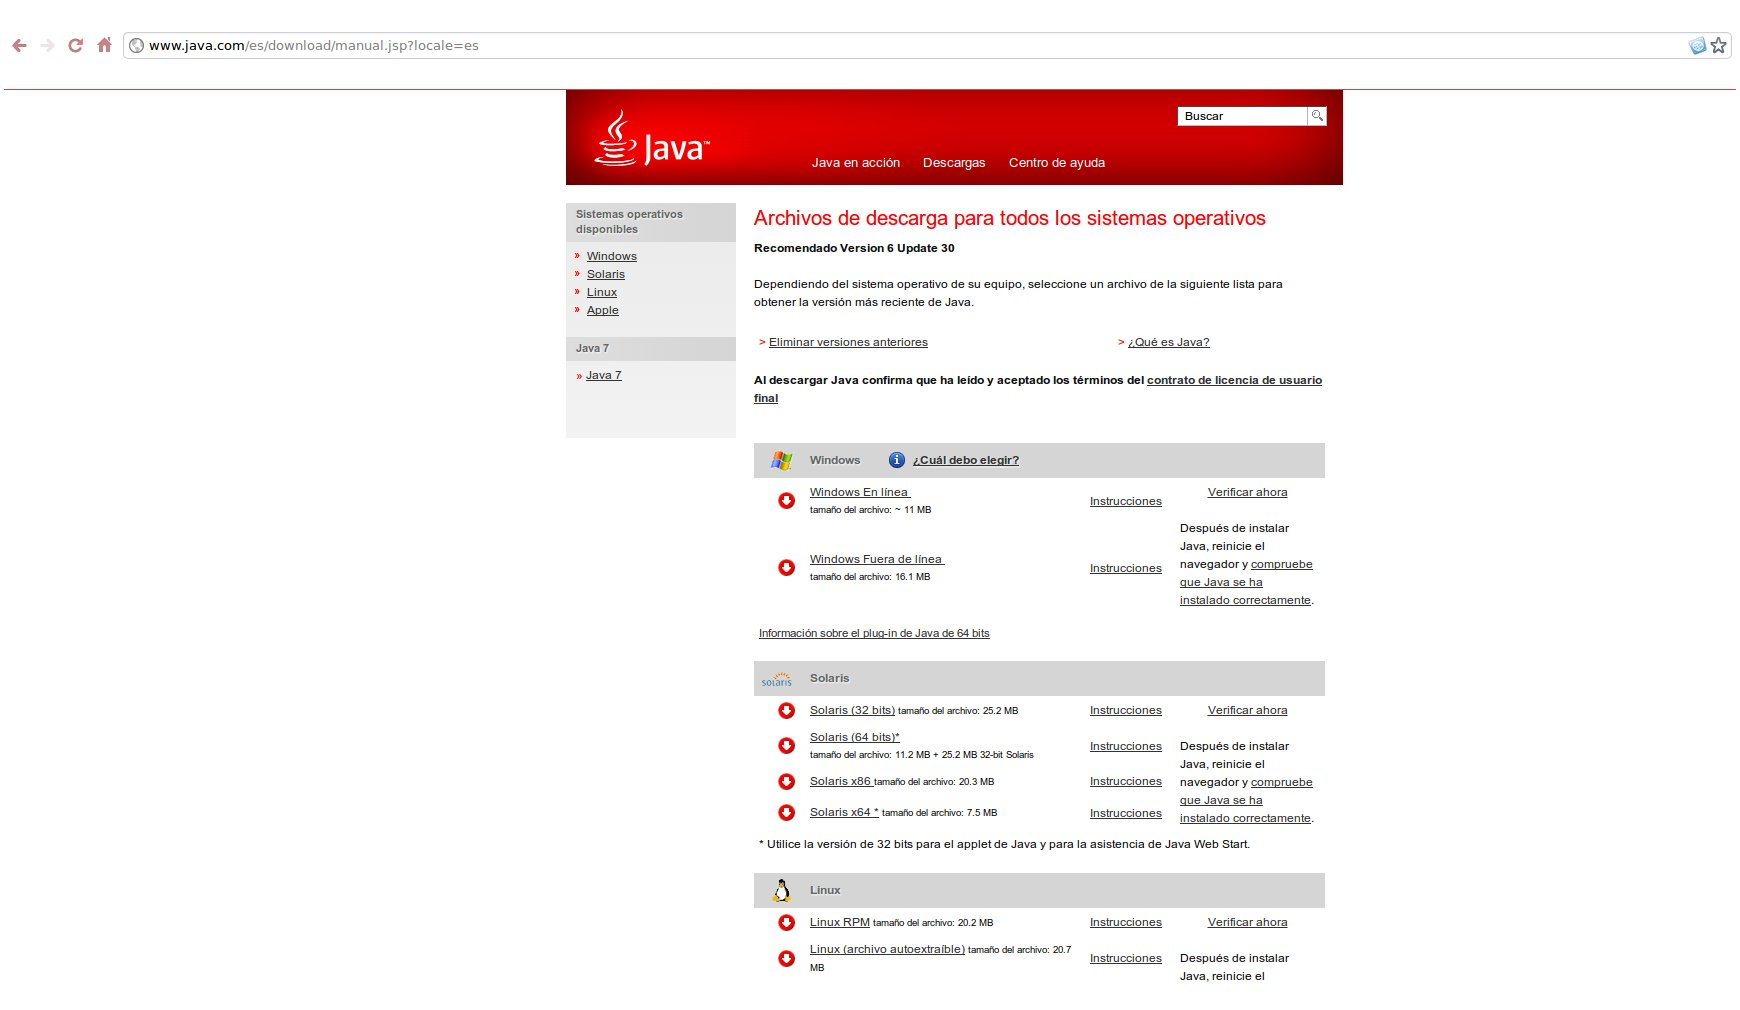
\includegraphics[width=20cm]{./imagenes_documentacion/captura_3.jpeg}}
\caption{Página web donde se encuentran los ficheros descargables según sistema operativo \url{http://www.java.com/es/download/manual.jsp?locale=es}}
\end{figure}

\begin{figure}[H]
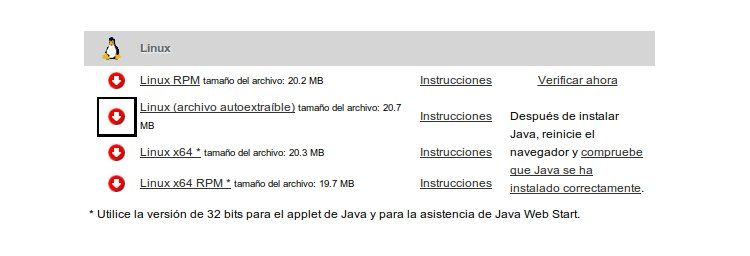
\includegraphics[width=15cm]{./imagenes_documentacion/captura_4.jpeg}
\caption{Sección de la página web de la figura 7.4 en donde se especifica para el sistema operativo GNU/Linux.}
\end{figure}

Si se desea la descarga del archivo en formato ``.rpm'' se deberá poner en la línea de comandos para su instalación el comando:\\

\begin{center} \emph{rpm -Uvh nombre\_paquete.rpm}\\ \end{center}

Si por el contrario se descarga el fichero en formato autoextraible será necesario escribir el siguiente comando en la línea de comandos:\\

\begin{center} \emph{sh nombre\_paquete.bin}\\ \end{center}

Además de todo ello se deberá tener instalado también el jdk de java para poder visualizar la aplicación perfectamente en nuestro sistema. Para ello tenemos que teclar en línea de comandos:\\
\begin{center} \emph{sudo apt-get install openjdk-jre} \\ \end{center}

\section{Operaciones de la suite}
\subsection{...}
\subsection{Menú principal}
\subsection{...}

\section{Índice}

